\documentclass[11pt,a4paper]{article}

% --- Packages ---
\usepackage[margin=1in]{geometry}
\usepackage{tikz}
\usetikzlibrary{
  arrows.meta,
  positioning,
  shapes.geometric,
  shapes.multipart,
  fit,
  calc,
  backgrounds,
  chains,
  decorations.pathreplacing,
  automata
}
\usepackage{listings}
\usepackage{xcolor}
\usepackage{hyperref}
\usepackage{amsmath,amssymb}
\usepackage{booktabs}
\usepackage{enumitem}
\usepackage{fancyhdr}
\usepackage{titlesec}
\usepackage{tcolorbox}
\tcbuselibrary{listings,skins,breakable}
\usepackage{graphicx}
\usepackage{float}
\usepackage{caption}

% --- Colors ---
\definecolor{cnblue}{HTML}{1A3A5C}
\definecolor{cnlight}{HTML}{4A90D9}
\definecolor{cngray}{HTML}{F5F5F5}
\definecolor{cngreen}{HTML}{2E7D32}
\definecolor{cnred}{HTML}{C62828}
\definecolor{cnorange}{HTML}{E65100}
\definecolor{cnpurple}{HTML}{6A1B9A}

% --- Code listing style ---
\lstdefinestyle{typescript}{
  language=Java,
  basicstyle=\ttfamily\footnotesize,
  keywordstyle=\color{cnblue}\bfseries,
  stringstyle=\color{cngreen},
  commentstyle=\color{gray}\itshape,
  breaklines=true,
  frame=none,
  showstringspaces=false,
  tabsize=2,
  morekeywords={async,await,const,let,interface,type,export,import,from,extends,
    implements,readonly,string,number,boolean,void,Promise,Map,undefined},
  literate={=>}{{\textcolor{cnblue}{=>}}}{2}
}

\lstdefinestyle{protobuf}{
  basicstyle=\ttfamily\footnotesize,
  keywordstyle=\color{cnblue}\bfseries,
  stringstyle=\color{cngreen},
  commentstyle=\color{gray}\itshape,
  breaklines=true,
  frame=none,
  showstringspaces=false,
  morekeywords={message,optional,repeated,string,uint32,bytes,enum,map,import,syntax,package}
}

% --- Code box environment ---
\newtcblisting{codebox}[2][]{
  colback=cngray,
  colframe=cnblue!60,
  listing only,
  listing options={style=#2,#1},
  left=6pt,
  right=6pt,
  top=4pt,
  bottom=4pt,
  boxrule=0.5pt,
  breakable
}

% --- Definition box ---
\newtcolorbox{defbox}[1]{
  colback=cnblue!5,
  colframe=cnblue!60,
  fonttitle=\bfseries,
  title=#1,
  boxrule=0.5pt
}

% --- Header/Footer ---
\pagestyle{fancy}
\fancyhf{}
\fancyhead[L]{\small\textcolor{cnblue}{DED Agent WorldState}}
\fancyhead[R]{\small\textcolor{cnblue}{Technical Proposal}}
\fancyfoot[C]{\thepage}
\renewcommand{\headrulewidth}{0.4pt}

% --- Title formatting ---
\titleformat{\section}{\Large\bfseries\color{cnblue}}{\thesection}{1em}{}
\titleformat{\subsection}{\large\bfseries\color{cnblue!80}}{\thesubsection}{1em}{}
\titleformat{\subsubsection}{\normalsize\bfseries\color{cnblue!60}}{\thesubsubsection}{1em}{}

% --- Document ---
\begin{document}

% --- Title Page ---
\begin{titlepage}
\centering
\vspace*{2cm}

{\Huge\bfseries\color{cnblue} DED Agent WorldState\par}
\vspace{0.5cm}
{\Large\color{cnblue!70} Verifiable Internal State for Autonomous Agents\par}
\vspace{1cm}
{\large Technical Proposal --- v0.1\par}
\vspace{0.5cm}
{\large\today\par}

\vspace{2cm}

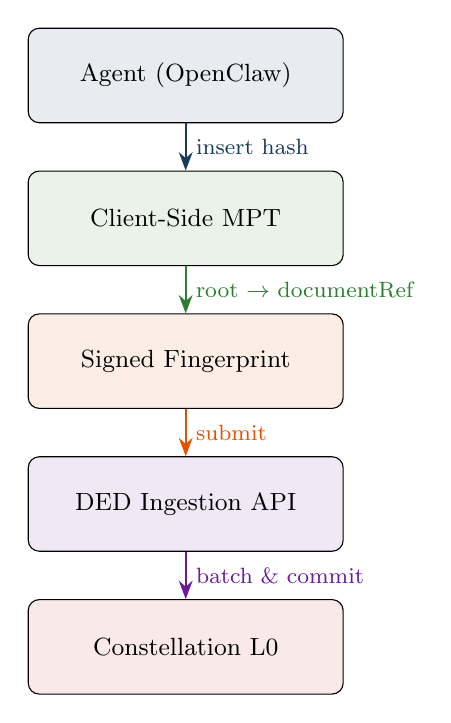
\begin{tikzpicture}[
  node distance=0.6cm,
  every node/.style={font=\small}
]
  % Agent box
  \node[draw, rounded corners, fill=cnblue!10, minimum width=4cm, minimum height=1.2cm]
    (agent) {Agent (OpenClaw)};

  % MPT box
  \node[draw, rounded corners, fill=cngreen!10, minimum width=4cm, minimum height=1.2cm,
    below=of agent] (mpt) {Client-Side MPT};

  % Fingerprint
  \node[draw, rounded corners, fill=cnorange!10, minimum width=4cm, minimum height=1.2cm,
    below=of mpt] (fp) {Signed Fingerprint};

  % DED
  \node[draw, rounded corners, fill=cnpurple!10, minimum width=4cm, minimum height=1.2cm,
    below=of fp] (ded) {DED Ingestion API};

  % L0
  \node[draw, rounded corners, fill=cnred!10, minimum width=4cm, minimum height=1.2cm,
    below=of ded] (l0) {Constellation L0};

  % Arrows
  \draw[-{Stealth}, thick, cnblue] (agent) -- node[right, font=\footnotesize] {insert hash} (mpt);
  \draw[-{Stealth}, thick, cngreen] (mpt) -- node[right, font=\footnotesize] {root $\to$ documentRef} (fp);
  \draw[-{Stealth}, thick, cnorange] (fp) -- node[right, font=\footnotesize] {submit} (ded);
  \draw[-{Stealth}, thick, cnpurple] (ded) -- node[right, font=\footnotesize] {batch \& commit} (l0);
\end{tikzpicture}

\vspace{2cm}

\begin{tabular}{ll}
\textbf{Status:} & Draft \\
\textbf{Authors:} & Constellation Network Engineering \\
\textbf{Package:} & \texttt{ded-agent-worldstate} (npm) \\
\textbf{Dependencies:} & \texttt{@constellation-network/ded-sdk}, \texttt{@constellation-network/metagraph-sdk} \\
\end{tabular}

\end{titlepage}

\tableofcontents
\newpage

% ============================================================================
\section{Motivation}
% ============================================================================

Autonomous AI agents are increasingly deployed to make decisions, execute workflows, and
interact with external systems on behalf of their operators. As agents gain autonomy, a
critical question emerges: \textbf{how can an agent prove what it knew, decided, or did at
any point in time?}

Today, agent state is ephemeral. Conversation logs, decision records, and internal
computations exist only in the agent's local memory or in opaque platform logs. There is no
cryptographic guarantee that the agent's reported history is complete, unmodified, or
temporally ordered. This creates trust gaps in three domains:

\begin{enumerate}[leftmargin=2cm]
  \item \textbf{Accountability} --- An agent that makes financial, legal, or safety-critical
    decisions cannot prove the reasoning chain that led to those decisions.
  \item \textbf{Compliance} --- Regulatory frameworks increasingly require auditable records
    of automated decision-making (e.g., EU AI Act, SEC algorithmic trading rules).
  \item \textbf{Inter-Agent Trust} --- When agents collaborate, there is no mechanism for
    one agent to verify another's claimed state without direct access to its internals.
\end{enumerate}

The \textbf{Digital Evidence Depository (DED)} provides a production-grade notarization
engine backed by the Constellation Network's Hypergraph. By combining the DED's fingerprint
submission pipeline with a client-side \textbf{Merkle Patricia Trie (MPT)}, we can give
agents a \emph{verifiable internal world state} --- a tamper-evident, temporally ordered,
cryptographically committed record of every state transition the agent makes.

% ============================================================================
\section{Use Cases}
% ============================================================================

\subsection{AI Reasoning Audit Trail}

An AI agent processing insurance claims notarizes each decision point: document receipt,
risk assessment, approval/denial, and payout authorization. Each decision is hashed and
inserted into the agent's world state trie. If a decision is later disputed, the agent can
produce an MPT inclusion proof demonstrating that the decision existed in its state at a
specific ordinal, with a corresponding on-chain commitment timestamp.

\subsection{Automated Compliance Monitoring}

A compliance agent monitors data streams for regulatory violations. Each detected event
(or clean-check confirmation) is recorded as a state entry. The chain of fingerprints
provides a tamper-evident log that auditors can independently verify against the
Constellation L0 without requiring access to the agent's infrastructure.

\subsection{Multi-Step Workflow Orchestration}

A workflow agent orchestrates a multi-party approval process (e.g., contract signing,
supply chain handoffs). Each state transition --- initiation, approval, counter-signature,
finalization --- is committed to the world state. The ordered chain of MPT roots provides a
verifiable timeline of the workflow's progression.

% ============================================================================
\section{System Architecture}
% ============================================================================

The system operates as a \textbf{two-level commitment architecture}:

\begin{enumerate}
  \item \textbf{Client-Level}: The agent maintains a per-stream MPT. Each state update
    inserts a hash into the trie, producing a new root. This root becomes the
    \texttt{documentRef} of a signed fingerprint.
  \item \textbf{Platform-Level}: The DED server batches fingerprints into its own
    server-side MPT, whose root is committed to the Constellation L0 blockchain via a
    \texttt{MetagraphBatchMessage}.
\end{enumerate}

\subsection{Architecture Diagram}

\begin{figure}[H]
\centering
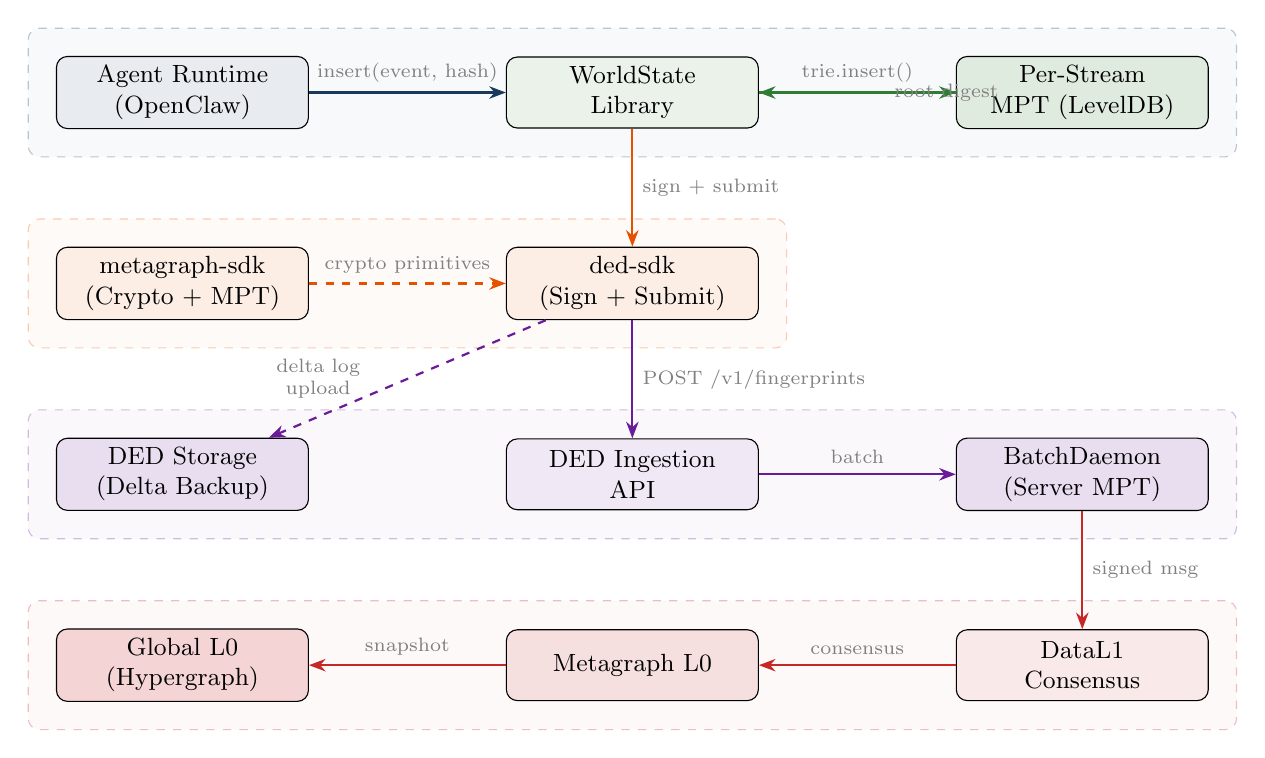
\begin{tikzpicture}[
  node distance=1.2cm and 2cm,
  box/.style={draw, rounded corners=4pt, minimum width=3.2cm, minimum height=0.9cm,
    font=\small, align=center},
  arrow/.style={-{Stealth[length=6pt]}, thick},
  label/.style={font=\scriptsize, text=gray}
]

  % --- Agent Layer ---
  \node[box, fill=cnblue!10] (agent) {Agent Runtime\\(OpenClaw)};
  \node[box, fill=cngreen!10, right=2.5cm of agent] (ws) {WorldState\\Library};
  \node[box, fill=cngreen!15, right=2.5cm of ws] (mpt) {Per-Stream\\MPT (LevelDB)};

  % --- SDK Layer ---
  \node[box, fill=cnorange!10, below=1.5cm of ws] (dedsdk) {ded-sdk\\(Sign + Submit)};
  \node[box, fill=cnorange!10, left=2.5cm of dedsdk] (metakit) {metagraph-sdk\\(Crypto + MPT)};

  % --- Server Layer ---
  \node[box, fill=cnpurple!10, below=1.5cm of dedsdk] (ingestion) {DED Ingestion\\API};
  \node[box, fill=cnpurple!15, right=2.5cm of ingestion] (batch) {BatchDaemon\\(Server MPT)};
  \node[box, fill=cnpurple!15, left=2.5cm of ingestion] (storage) {DED Storage\\(Delta Backup)};

  % --- Chain Layer ---
  \node[box, fill=cnred!10, below=1.5cm of batch] (dl1) {DataL1\\Consensus};
  \node[box, fill=cnred!15, left=2.5cm of dl1] (ml0) {Metagraph L0};
  \node[box, fill=cnred!20, left=2.5cm of ml0] (gl0) {Global L0\\(Hypergraph)};

  % --- Arrows: Agent Layer ---
  \draw[arrow, cnblue] (agent) -- node[above, label] {insert(event, hash)} (ws);
  \draw[arrow, cngreen] (ws) -- node[above, label] {trie.insert()} (mpt);
  \draw[arrow, cngreen, dashed] (mpt) -- node[right, label, text width=2cm, align=center]
    {root digest} (ws);

  % --- Arrows: SDK Layer ---
  \draw[arrow, cnorange] (ws) -- node[right, label] {sign + submit} (dedsdk);
  \draw[arrow, cnorange, dashed] (metakit) -- node[above, label] {crypto primitives} (dedsdk);

  % --- Arrows: Server Layer ---
  \draw[arrow, cnpurple] (dedsdk) -- node[right, label] {POST /v1/fingerprints} (ingestion);
  \draw[arrow, cnpurple] (ingestion) -- node[above, label] {batch} (batch);
  \draw[arrow, cnpurple, dashed] (dedsdk) -- node[left, label, text width=2cm, align=center]
    {delta log\\upload} (storage);

  % --- Arrows: Chain Layer ---
  \draw[arrow, cnred] (batch) -- node[right, label] {signed msg} (dl1);
  \draw[arrow, cnred] (dl1) -- node[above, label] {consensus} (ml0);
  \draw[arrow, cnred] (ml0) -- node[above, label] {snapshot} (gl0);

  % --- Background boxes ---
  \begin{scope}[on background layer]
    \node[draw=cnblue!30, dashed, rounded corners, fill=cnblue!3,
      fit=(agent)(ws)(mpt), inner sep=10pt, label={[font=\footnotesize\bfseries,
      text=cnblue]above:Agent Layer}] {};
    \node[draw=cnorange!30, dashed, rounded corners, fill=cnorange!3,
      fit=(metakit)(dedsdk), inner sep=10pt, label={[font=\footnotesize\bfseries,
      text=cnorange]above:SDK Layer}] {};
    \node[draw=cnpurple!30, dashed, rounded corners, fill=cnpurple!3,
      fit=(storage)(ingestion)(batch), inner sep=10pt, label={[font=\footnotesize\bfseries,
      text=cnpurple]above:DED Server Layer}] {};
    \node[draw=cnred!30, dashed, rounded corners, fill=cnred!3,
      fit=(gl0)(ml0)(dl1), inner sep=10pt, label={[font=\footnotesize\bfseries,
      text=cnred]above:Constellation Network}] {};
  \end{scope}
\end{tikzpicture}
\caption{Four-layer system architecture. The agent inserts state hashes into a local MPT,
commits roots as fingerprints via the DED SDK, which are batched and committed on-chain.}
\label{fig:architecture}
\end{figure}


% ============================================================================
\section{Data Model}
% ============================================================================

\subsection{Extended FingerprintValue}

The \texttt{FingerprintValue} protobuf message is extended with two optional fields:

\begin{codebox}{protobuf}
message FingerprintValue {
  string org_id = 1;
  string tenant_id = 2;
  string event_id = 3;
  optional string signer_id = 4;
  string document_id = 5;
  string document_ref = 6;
  Timestamp timestamp = 7;
  uint32 version = 8;

  // NEW: Stream routing fields
  optional string stream_id = 9;   // UUID v4
  optional string app_id = 10;     // UUID v4
}
\end{codebox}

\begin{itemize}
  \item \texttt{stream\_id} and \texttt{app\_id} are \textbf{optional} with a default of
    the zero UUID (\texttt{00000000-0000-0000-0000-000000000000}) when omitted.
  \item This preserves \textbf{backwards compatibility} --- existing clients that do not
    set these fields continue to work unchanged.
  \item The SDK transparently applies the default when constructing fingerprint values.
\end{itemize}

\subsection{Data Structure Diagram}

\begin{figure}[H]
\centering
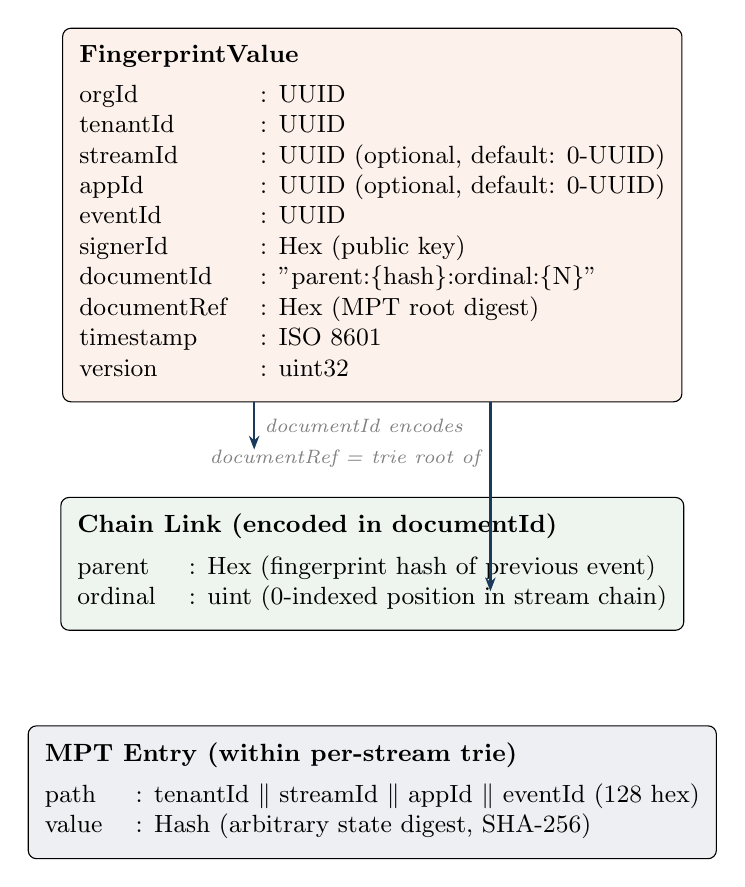
\begin{tikzpicture}[
  record/.style={draw, rounded corners=3pt, minimum width=7cm, font=\small,
    inner sep=6pt, align=left},
  field/.style={font=\ttfamily\scriptsize},
  arrow/.style={-{Stealth[length=5pt]}, thick, cnblue},
  note/.style={font=\scriptsize\itshape, text=gray}
]

  % FingerprintValue
  \node[record, fill=cnorange!8] (fpv) {
    \textbf{FingerprintValue} \\[4pt]
    \begin{tabular}{@{}ll@{}}
      \field{orgId}       & \field{: UUID} \\
      \field{tenantId}    & \field{: UUID} \\
      \field{streamId}    & \field{: UUID (optional, default: 0-UUID)} \\
      \field{appId}       & \field{: UUID (optional, default: 0-UUID)} \\
      \field{eventId}     & \field{: UUID} \\
      \field{signerId}    & \field{: Hex (public key)} \\
      \field{documentId}  & \field{: "parent:\{hash\}:ordinal:\{N\}"} \\
      \field{documentRef} & \field{: Hex (MPT root digest)} \\
      \field{timestamp}   & \field{: ISO 8601} \\
      \field{version}     & \field{: uint32} \\
    \end{tabular}
  };

  % Chain link annotation
  \node[record, fill=cngreen!8, below=1.2cm of fpv] (chain) {
    \textbf{Chain Link (encoded in documentId)} \\[4pt]
    \begin{tabular}{@{}ll@{}}
      \field{parent}  & \field{: Hex (fingerprint hash of previous event)} \\
      \field{ordinal} & \field{: uint (0-indexed position in stream chain)} \\
    \end{tabular}
  };

  % MPT Entry
  \node[record, fill=cnblue!8, below=1.2cm of chain] (entry) {
    \textbf{MPT Entry (within per-stream trie)} \\[4pt]
    \begin{tabular}{@{}ll@{}}
      \field{path}  & \field{: tenantId $\|$ streamId $\|$ appId $\|$ eventId (128 hex)} \\
      \field{value} & \field{: Hash (arbitrary state digest, SHA-256)} \\
    \end{tabular}
  };

  % Arrows
  \draw[arrow] (fpv.south) +(-1.5,0) -- +(-1.5,-0.6)
    node[right, note, pos=0.5] {documentId encodes};
  \draw[arrow] (fpv.south) +(1.5,0) -- +(1.5,-2.4)
    node[left, note, pos=0.3] {documentRef = trie root of};

\end{tikzpicture}
\caption{Relationship between FingerprintValue fields, chain linking, and MPT entries.}
\label{fig:datamodel}
\end{figure}

\subsection{Evidence Path Construction}

The MPT key path is constructed by concatenating four UUIDs as raw bytes, then
hex-encoding:

\[
  \text{path} = \text{hex}(\text{tenantId}_{16\text{B}} \| \text{streamId}_{16\text{B}}
  \| \text{appId}_{16\text{B}} \| \text{eventId}_{16\text{B}}) = 128 \text{ hex chars}
\]

This matches the server-side \texttt{PathEvidenceCalculator} format, ensuring that the
client-side and server-side MPT paths are structurally aligned. The SDK enforces this
invariant; the server treats \texttt{documentRef} as opaque.

\subsection{Chain Linking Protocol}

Each fingerprint in a stream carries a \texttt{documentId} that encodes its position in
the revision chain:

\begin{defbox}{documentId Format}
\texttt{parent:\{fingerprint\_hash\}:ordinal:\{N\}}
\end{defbox}

\begin{itemize}
  \item \textbf{Genesis event}: \texttt{parent:genesis:ordinal:0}
  \item \textbf{Subsequent events}: \texttt{parent:\{sha256\_hash\}:ordinal:\{N+1\}}
  \item The \texttt{fingerprint\_hash} is the authoritative hash returned by the DED API
    upon successful submission of the previous event.
  \item Chain integrity: the agent waits for the API response (synchronous mode) before
    constructing the next link.
\end{itemize}

% ============================================================================
\section{State Update Lifecycle}
% ============================================================================

\noindent
\begin{minipage}{\textwidth}
\centering
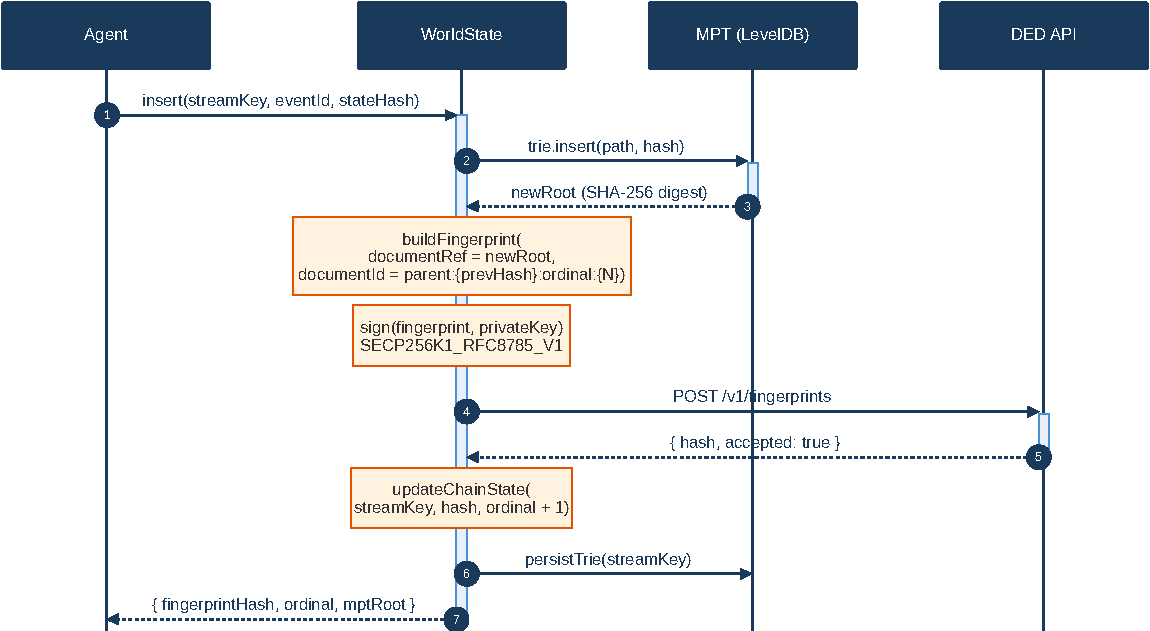
\includegraphics[width=0.78\textwidth,keepaspectratio]{fig-sequence-cropped.pdf}
\captionof{figure}{Sequence diagram for a single state update.}
\label{fig:sequence}
\end{minipage}

\medskip\noindent
The complete lifecycle of a single state insertion (Figure~\ref{fig:sequence}):

\begin{enumerate}[nosep,leftmargin=1.5cm]
  \item \textbf{Agent calls} \texttt{worldState.insert(streamKey, eventId, stateHash)}
  \item \textbf{WorldState} constructs the 128-hex-char MPT path from the stream key
    components and eventId
  \item \textbf{MPT.insert} adds the \texttt{(path, stateHash)} entry to the per-stream
    trie and computes the new root digest
  \item \textbf{WorldState} constructs a \texttt{FingerprintValue} with
    \texttt{documentRef} = new MPT root,
    \texttt{documentId} = \texttt{parent:\{prevHash\}:ordinal:\{N\}},
    and \texttt{streamId}/\texttt{appId}/\texttt{eventId} from the stream key
  \item \textbf{Sign} the fingerprint using SECP256K1\_RFC8785\_V1 with the agent's
    private key
  \item \textbf{Submit} to DED Ingestion API; \textbf{block} until response
  \item \textbf{On success}: update local chain state (new parent hash, increment ordinal),
    persist trie to LevelDB
  \item \textbf{Return} the fingerprint hash to the agent
\end{enumerate}


% ============================================================================
\section{Stream State Machine}
% ============================================================================

\begin{figure}[H]
\centering
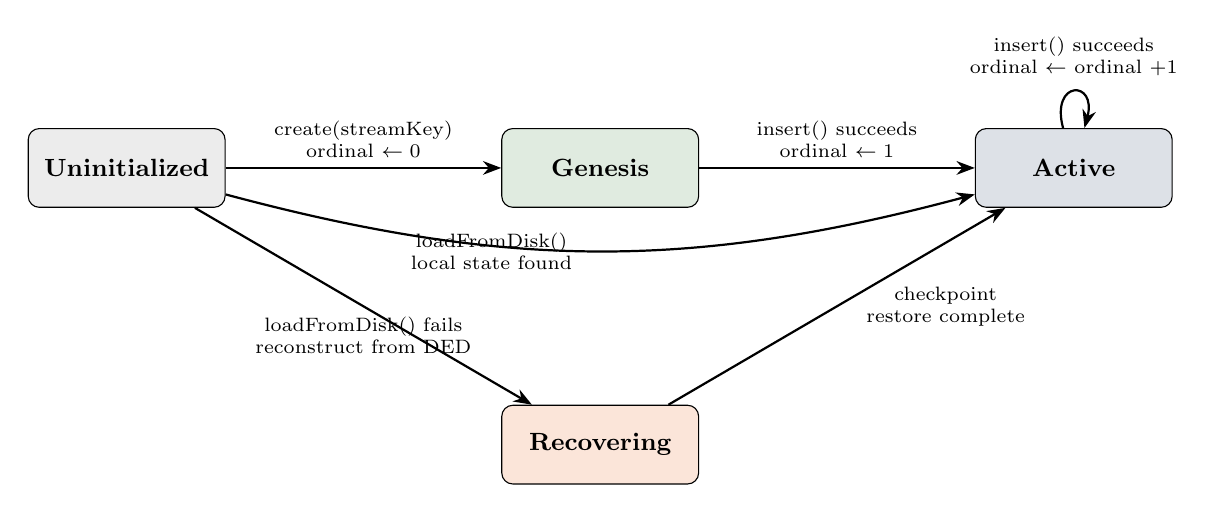
\begin{tikzpicture}[
  ->,
  >=Stealth,
  node distance=3.5cm,
  state/.style={draw, rounded corners=4pt, minimum width=2.5cm, minimum height=1cm,
    font=\small\bfseries, align=center},
  every edge/.style={draw, thick},
  label/.style={font=\scriptsize, align=center}
]

  \node[state, fill=gray!15] (uninit) {Uninitialized};
  \node[state, fill=cngreen!15, right=of uninit] (genesis) {Genesis};
  \node[state, fill=cnblue!15, right=of genesis] (active) {Active};

  % Recovery states
  \node[state, fill=cnorange!15, below=2.5cm of genesis] (recovering) {Recovering};

  % Transitions
  \draw (uninit) edge[above] node[label] {create(streamKey)\\ordinal $\gets 0$} (genesis);
  \draw (genesis) edge[above] node[label] {insert() succeeds\\ordinal $\gets 1$} (active);
  \draw (active) edge[loop above, looseness=6] node[label, above=2pt]
    {insert() succeeds\\ordinal $\gets$ ordinal $+ 1$} (active);

  \draw (uninit) edge[bend right=15, left] node[label, text width=2.5cm]
    {loadFromDisk()\\local state found} (active);
  \draw (uninit) edge[below] node[label, text width=3cm]
    {loadFromDisk() fails\\reconstruct from DED} (recovering);
  \draw (recovering) edge[right] node[label, text width=2.5cm]
    {checkpoint\\restore complete} (active);

\end{tikzpicture}
\caption{Stream lifecycle state machine. Streams are always open once active. Recovery
restores from the latest checkpoint and replays subsequent entries.}
\label{fig:statemachine}
\end{figure}

\begin{itemize}
  \item \textbf{Uninitialized}: Stream has not been created or loaded.
  \item \textbf{Genesis}: First event pending. \texttt{documentId} will be
    \texttt{parent:genesis:ordinal:0}.
  \item \textbf{Active}: Stream is accepting insertions. Each successful insertion
    increments the ordinal and updates the parent hash.
  \item \textbf{Recovering}: Local state was lost. The library downloads the latest
    checkpoint from DED Storage and replays any subsequent entries to reconstruct the trie.
  \item Streams are \textbf{always open} --- there is no sealed/closed state.
\end{itemize}


% ============================================================================
\section{Checkpoint-Based Recovery}
% ============================================================================

\subsection{Design Constraint}

The DED storage system enforces that when a fingerprint includes a document payload, the
\texttt{documentRef} must equal the SHA-256 hash of that payload. Since WorldState
fingerprints use \texttt{documentRef} for the MPT root digest, delta entries \emph{cannot}
be attached as payloads to the same fingerprint submission. Instead, trie backups are
performed as separate \textbf{checkpoint jobs}.

\subsection{Checkpoint Model}

The agent periodically exports a full snapshot of the trie's entries as a separate
fingerprint submission dedicated to backup:

\begin{codebox}{typescript}
interface TrieCheckpoint {
  streamKey: StreamKey;       // (tenantId, streamId, appId)
  entries: Record<string, string>;  // path -> hash (all trie entries)
  asOfOrdinal: number;       // Chain ordinal at time of checkpoint
  asOfMptRoot: string;       // MPT root at time of checkpoint
}
\end{codebox}

\textbf{Checkpoint submission:}
\begin{itemize}
  \item The serialized checkpoint is uploaded to DED Storage as a document payload.
  \item Its \texttt{documentRef} = SHA-256 of the serialized checkpoint (satisfying the
    storage constraint).
  \item A dedicated \texttt{documentId} format distinguishes checkpoints from state
    entries: \texttt{checkpoint:\{streamId\}:ordinal:\{N\}}.
  \item Checkpoints use their own stream (e.g., \texttt{appId = checkpoint-app-uuid}) to
    avoid polluting the primary state chain.
\end{itemize}

\subsection{Recovery Procedure}

\begin{enumerate}
  \item Query DED for the latest checkpoint fingerprint for this stream.
  \item Download the checkpoint payload from DED Storage.
  \item Deserialize the \texttt{TrieCheckpoint} and rebuild the MPT from its entries.
  \item Query the primary stream chain for any fingerprints with ordinal $>$
    \texttt{asOfOrdinal}.
  \item For each subsequent fingerprint, the agent needs the original
    \texttt{(path, stateHash)} to replay. If objects are stored externally (application
    database, S3, etc.), re-derive the entry and insert into the trie.
  \item Verify the reconstructed trie root matches the latest chain's \texttt{documentRef}.
\end{enumerate}

\subsection{Checkpoint Cost}

A stream with 10,000 entries produces a checkpoint of $\sim$2\,MB (128-char path + 64-char
hash per entry). At 1 credit per 100\,KB, this costs $\sim$20 credits (\$0.20) per
checkpoint plus 2 credits for the fingerprint write. Checkpointing frequency is
configurable --- e.g., every 1,000 insertions or daily.


% ============================================================================
\section{Verification Flow}
% ============================================================================

An agent can verify that a specific event exists in its committed world state through a
three-layer proof chain:

\begin{figure}[H]
\centering
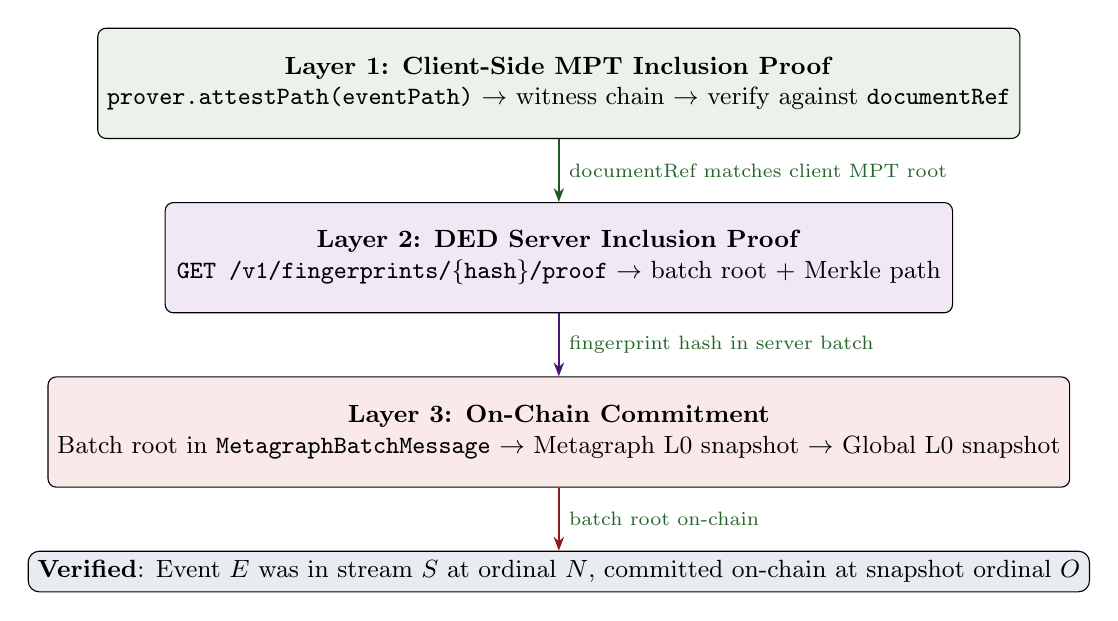
\begin{tikzpicture}[
  node distance=0.8cm,
  layer/.style={draw, rounded corners=3pt, minimum width=10cm, minimum height=1.4cm,
    font=\small, align=center},
  arrow/.style={-{Stealth[length=5pt]}, thick},
  check/.style={font=\scriptsize, text=cngreen!80!black}
]

  % Layer 1: Client MPT
  \node[layer, fill=cngreen!10] (l1) {
    \textbf{Layer 1: Client-Side MPT Inclusion Proof} \\
    \texttt{prover.attestPath(eventPath)} $\to$ witness chain $\to$ verify against
    \texttt{documentRef}
  };

  % Layer 2: Server MPT
  \node[layer, fill=cnpurple!10, below=of l1] (l2) {
    \textbf{Layer 2: DED Server Inclusion Proof} \\
    \texttt{GET /v1/fingerprints/\{hash\}/proof} $\to$ batch root + Merkle path
  };

  % Layer 3: On-chain
  \node[layer, fill=cnred!10, below=of l2] (l3) {
    \textbf{Layer 3: On-Chain Commitment} \\
    Batch root in \texttt{MetagraphBatchMessage} $\to$ Metagraph L0 snapshot $\to$
    Global L0 snapshot
  };

  % Arrows
  \draw[arrow, cngreen!70!black] (l1) -- node[right, check]
    {documentRef matches client MPT root} (l2);
  \draw[arrow, cnpurple!70!black] (l2) -- node[right, check]
    {fingerprint hash in server batch} (l3);

  % Verification result
  \node[draw, rounded corners, fill=cnblue!10, minimum width=10cm, font=\small,
    below=of l3] (result) {
    \textbf{Verified}: Event $E$ was in stream $S$ at ordinal $N$, committed on-chain at
    snapshot ordinal $O$
  };
  \draw[arrow, cnred!70!black] (l3) -- node[right, check] {batch root on-chain} (result);

\end{tikzpicture}
\caption{Three-layer verification flow. Each layer's output anchors the layer above it.}
\label{fig:verification}
\end{figure}

\textbf{Key property}: Verification at Layer 1 requires the client's trie (or a
reconstructed copy). Layers 2 and 3 are publicly verifiable using only the fingerprint hash
and the DED/Constellation public APIs.


% ============================================================================
\section{API Surface}
% ============================================================================

\begin{codebox}{typescript}
import { WorldState } from 'ded-agent-worldstate';

// --- Initialization ---
const ws = await WorldState.create({
  privateKey: '...',           // SECP256K1 private key (hex)
  orgId: 'org-uuid',
  baseUrl: 'https://api.ded.example.com',
  apiKey: 'your-api-key',
  storagePath: './worldstate', // LevelDB directory
});

// --- Define a stream ---
const stream = ws.stream({
  tenantId: 'tenant-uuid',
  streamId: 'stream-uuid',
  appId: 'app-uuid',
});

// --- Insert state ---
const eventId = crypto.randomUUID();
const stateHash = sha256(canonicalize(myStateObject));
const result = await stream.insert(eventId, stateHash);
// result: { fingerprintHash, ordinal, mptRoot }

// --- Verify inclusion ---
const proof = await stream.prove(eventId);
// proof: { clientProof: MerklePatriciaInclusionProof, fingerprintHash }

const isValid = await stream.verify(proof);
// isValid: true

// --- Inspect state ---
const info = await stream.info();
// info: { ordinal, latestRoot, latestFingerprintHash, entryCount }

// --- Checkpoint (backup) ---
await stream.checkpoint();
// Serializes trie entries, uploads to DED Storage

// --- Recovery (from checkpoint) ---
const recovered = await stream.recover();
// Downloads latest checkpoint, replays subsequent entries
\end{codebox}


% ============================================================================
\section{OpenClaw Integration Example}
% ============================================================================

The following shows a complete OpenClaw AgentSkill that uses the WorldState library to
notarize agent decisions:

\begin{codebox}{typescript}
// SKILL.md frontmatter (YAML):
// ---
// name: ded-worldstate
// description: Notarize agent decisions to DED
// version: 1.0.0
// metadata:
//   openclaw:
//     emoji: "🔏"
//     bins: [node]
//     env: [DED_API_KEY, DED_PRIVATE_KEY, DED_ORG_ID]
//     os: [darwin, linux]
// ---

import { WorldState } from 'ded-agent-worldstate';
import { sha256, canonicalize } from '@constellation-network/metagraph-sdk';

const ws = await WorldState.create({
  privateKey: process.env.DED_PRIVATE_KEY!,
  orgId: process.env.DED_ORG_ID!,
  baseUrl: 'https://ded-api.constellationnetwork.io',
  apiKey: process.env.DED_API_KEY!,
  storagePath: `${process.env.HOME}/.openclaw/worldstate`,
});

// Create a stream for this agent's decision log
const decisions = ws.stream({
  tenantId: 'my-tenant-uuid',
  streamId: 'decisions-stream-uuid',
  appId: 'openclaw-skill-uuid',
});

// Skill handler: notarize a decision
export async function notarizeDecision(context: {
  action: string;
  reasoning: string;
  confidence: number;
  inputs: Record<string, unknown>;
}) {
  const stateHash = sha256(canonicalize(context));
  const eventId = crypto.randomUUID();

  const result = await decisions.insert(eventId, stateHash);

  return {
    message: `Decision notarized at ordinal ${result.ordinal}`,
    fingerprintHash: result.fingerprintHash,
    mptRoot: result.mptRoot,
    eventId,
  };
}

// Skill handler: verify a past decision
export async function verifyDecision(eventId: string) {
  const proof = await decisions.prove(eventId);
  const valid = await decisions.verify(proof);

  return {
    verified: valid,
    proof: proof.clientProof,
    fingerprintHash: proof.fingerprintHash,
  };
}
\end{codebox}


% ============================================================================
\section{Cost Analysis}
% ============================================================================

\begin{table}[H]
\centering
\begin{tabular}{@{}lrrr@{}}
\toprule
\textbf{Operation} & \textbf{Credits} & \textbf{Cost (USD)} & \textbf{Notes} \\
\midrule
Fingerprint write     & 2 & \$0.02 & Per state insertion \\
Authenticated read    & 1 & \$0.01 & Filtered search, tags returned \\
Public read           & 0 & Free   & Fingerprint value only \\
Storage write         & 1/100\,KB & \$0.01/100\,KB & For checkpoint uploads \\
\midrule
\textbf{Per insertion} & \textbf{2} & \textbf{\$0.02} & Fingerprint only \\
\bottomrule
\end{tabular}
\caption{Per-operation cost breakdown. Credits are \$0.01 each. Checkpoints are separate.}
\label{tab:costs}
\end{table}

\begin{table}[H]
\centering
\begin{tabular}{@{}lrrrr@{}}
\toprule
\textbf{Scenario} & \textbf{Events/day} & \textbf{Daily Cost} & \textbf{Monthly Cost}
  & \textbf{Checkpoint} \\
\midrule
Low-frequency agent   & 10    & \$0.20    & \$6     & \$0.22/wk \\
Moderate agent        & 100   & \$2.00    & \$60    & \$0.22/day \\
High-frequency agent  & 1,000 & \$20.00   & \$600   & \$0.22/day \\
\bottomrule
\end{tabular}
\caption{Projected costs by agent activity level. Checkpoint cost assumes $\sim$2\,MB
snapshot ($\sim$10K entries) = 20 storage credits + 2 fingerprint credits.}
\label{tab:scenarios}
\end{table}

\textbf{Checkpoint cost}: A 10,000-entry trie serializes to $\sim$2\,MB. At 1 credit per
100\,KB, a checkpoint costs $\sim$22 credits (\$0.22). Checkpointing every 1,000 insertions
or daily keeps recovery cost predictable. Recovery requires downloading the latest
checkpoint (1 read credit + storage download) and replaying only the entries since that
checkpoint.


% ============================================================================
\section{Threat Model}
% ============================================================================

\begin{figure}[H]
\centering
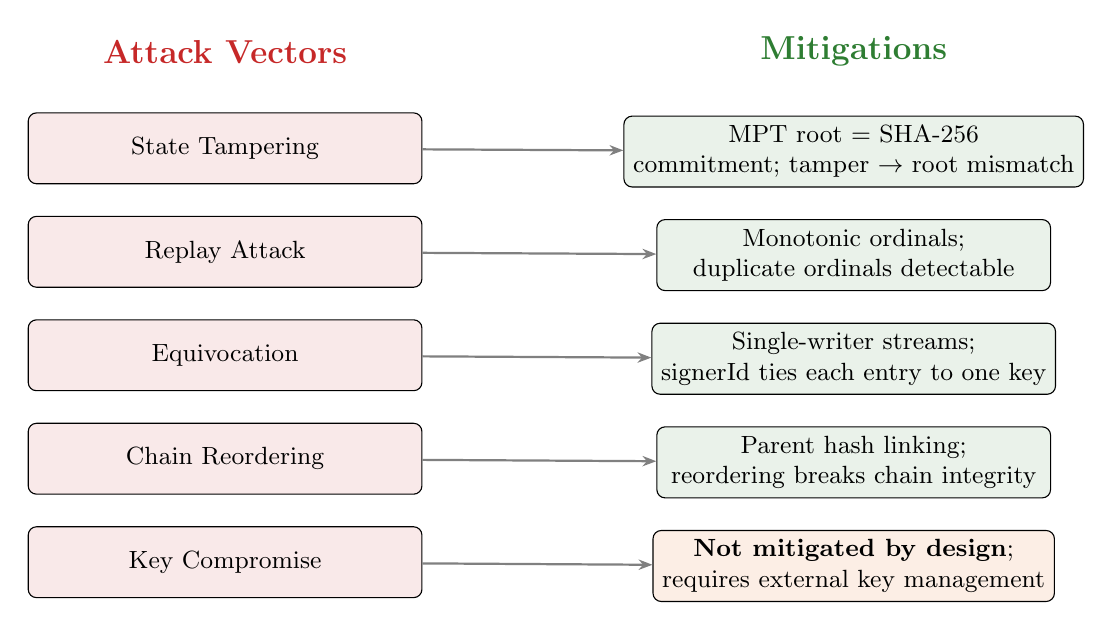
\begin{tikzpicture}[
  node distance=1.2cm,
  threat/.style={draw, rounded corners=3pt, minimum width=5cm, font=\small, align=center,
    minimum height=0.9cm},
  defense/.style={draw, rounded corners=3pt, minimum width=5cm, font=\small, align=center,
    minimum height=0.9cm},
  arrow/.style={-{Stealth[length=5pt]}, thick}
]

  \node[font=\large\bfseries, text=cnred] (title_t) {Attack Vectors};
  \node[font=\large\bfseries, text=cngreen, right=5cm of title_t] (title_d) {Mitigations};

  % Threats
  \node[threat, fill=cnred!10, below=0.5cm of title_t] (t1) {State Tampering};
  \node[threat, fill=cnred!10, below=0.4cm of t1] (t2) {Replay Attack};
  \node[threat, fill=cnred!10, below=0.4cm of t2] (t3) {Equivocation};
  \node[threat, fill=cnred!10, below=0.4cm of t3] (t4) {Chain Reordering};
  \node[threat, fill=cnred!10, below=0.4cm of t4] (t5) {Key Compromise};

  % Defenses
  \node[defense, fill=cngreen!10, below=0.5cm of title_d] (d1)
    {MPT root = SHA-256\\commitment; tamper $\to$ root mismatch};
  \node[defense, fill=cngreen!10, below=0.4cm of d1] (d2)
    {Monotonic ordinals;\\duplicate ordinals detectable};
  \node[defense, fill=cngreen!10, below=0.4cm of d2] (d3)
    {Single-writer streams;\\signerId ties each entry to one key};
  \node[defense, fill=cngreen!10, below=0.4cm of d3] (d4)
    {Parent hash linking;\\reordering breaks chain integrity};
  \node[defense, fill=cnorange!10, below=0.4cm of d4] (d5)
    {\textbf{Not mitigated by design};\\requires external key management};

  % Arrows
  \draw[arrow, gray] (t1) -- (d1);
  \draw[arrow, gray] (t2) -- (d2);
  \draw[arrow, gray] (t3) -- (d3);
  \draw[arrow, gray] (t4) -- (d4);
  \draw[arrow, gray] (t5) -- (d5);

\end{tikzpicture}
\caption{Threat model. The system defends against state tampering, replay, equivocation,
and reordering. Key compromise is explicitly out of scope.}
\label{fig:threats}
\end{figure}

\subsection{Security Properties}

\begin{description}[leftmargin=2cm, style=nextline]
  \item[Tamper Evidence]
    Any modification to a past state entry changes the MPT root, which is committed as
    \texttt{documentRef} in an immutable fingerprint. The on-chain commitment makes
    retroactive modification detectable.

  \item[Non-Repudiation]
    Each fingerprint carries an ECDSA signature from the agent's key (\texttt{signerId}).
    The agent cannot deny having submitted a state update without claiming key compromise.

  \item[Temporal Ordering]
    The \texttt{parent:\{hash\}:ordinal:\{N\}} chain enforces a total order on events
    within a stream. The DED server enforces monotonic timestamps per organization.

  \item[Inclusion Provability]
    Any event's presence in the world state can be proven via MPT inclusion proof without
    revealing other entries in the trie.
\end{description}

\subsection{Explicit Non-Goals}

\begin{itemize}
  \item \textbf{Confidentiality}: The system commits hashes, not plaintext. However,
    metadata (event IDs, timestamps, ordinals) is visible. If metadata confidentiality is
    required, additional encryption layers are needed.
  \item \textbf{Availability}: The system depends on the DED API and Constellation
    Network. Network outages prevent new commits but do not affect local state.
  \item \textbf{Key Management}: Secure storage and rotation of the agent's private key is
    the operator's responsibility.
\end{itemize}


% ============================================================================
\section{Vision: Agent-to-Agent Trust}
% ============================================================================

While the initial design focuses on \emph{self-verification} --- an agent proving the
integrity of its own state --- the architecture naturally extends to \emph{inter-agent
trust}:

\begin{enumerate}
  \item \textbf{Shared Trust Layer}: The DED serves as a neutral, publicly queryable
    commitment log. Agent A publishes its world state roots; Agent B can verify A's claims
    by checking the on-chain commitments without direct communication.

  \item \textbf{Cross-Agent Proofs}: If Agent A shares an MPT inclusion proof with Agent B
    (e.g., via DED Storage payloads), B can verify the proof against A's published
    \texttt{documentRef} without needing A's full trie.

  \item \textbf{Trust Chains}: Agent A can include Agent B's latest fingerprint hash in its
    own state entries, creating a cross-reference. This enables verifiable dependency
    chains across agents: ``A's decision at ordinal 5 was based on B's state at ordinal
    12.''

  \item \textbf{Reputation via Commitment History}: An agent's commitment history ---
    frequency, consistency, chain integrity --- becomes a verifiable reputation signal.
    Agents with long, unbroken commitment chains demonstrate operational reliability.
\end{enumerate}

This vision positions the DED not merely as a notarization service, but as a
\textbf{decentralized trust substrate for autonomous agent ecosystems}.


% ============================================================================
\section{Implementation Roadmap}
% ============================================================================

\begin{table}[H]
\centering
\begin{tabular}{@{}clp{7cm}@{}}
\toprule
\textbf{Phase} & \textbf{Deliverable} & \textbf{Description} \\
\midrule
1 & MPT Port (TypeScript) & Port \texttt{MerklePatriciaTrie}, \texttt{Producer},
  \texttt{Prover}, \texttt{Verifier} from metakit Scala to
  \texttt{@constellation-network/metagraph-sdk} TypeScript. Include shared test vectors for
  cross-language compatibility. \\[6pt]
2 & FingerprintValue Extension & Add \texttt{stream\_id} and \texttt{app\_id} to proto
  schema, ded-sdk types, and validation. Backwards-compatible (optional with defaults). \\[6pt]
3 & \texttt{ded-agent-worldstate} & Core library: \texttt{WorldState}, per-stream MPT
  management, chain linking, LevelDB persistence, DED API integration. \\[6pt]
4 & Checkpoint \& Recovery & DED Storage integration for periodic trie snapshot uploads.
  Recovery procedure: checkpoint download + incremental replay. \\[6pt]
5 & OpenClaw Skill Example & Reference OpenClaw AgentSkill demonstrating end-to-end
  integration. Published to ClawHub. \\
\bottomrule
\end{tabular}
\caption{Implementation phases. Each phase builds on the previous and is independently
testable.}
\label{tab:roadmap}
\end{table}


% ============================================================================
\section*{Appendix A: Server-Side Alignment}
% ============================================================================
\addcontentsline{toc}{section}{Appendix A: Server-Side Alignment}

The following server-side changes are required to fully support the extended schema and
stream-aware features. These are documented here for the DED server team and are
\textbf{not} part of the client-side implementation scope.

\subsection*{A.1 Protobuf Schema}

Add \texttt{stream\_id} (field 9) and \texttt{app\_id} (field 10) to
\texttt{DigitalEvidence\_v1.proto} as optional string fields with UUID validation rules.

\subsection*{A.2 Database Migration}

\begin{codebox}{typescript}
-- V<N>__add_stream_app_fields.sql
ALTER TABLE fingerprint_values
  ADD COLUMN stream_id UUID,
  ADD COLUMN app_id UUID;

CREATE INDEX idx_fpv_stream ON fingerprint_values (tenant_id, stream_id, app_id);
\end{codebox}

\subsection*{A.3 PathEvidenceCalculator}

Update to read \texttt{stream\_id} and \texttt{app\_id} from the fingerprint value instead
of defaulting to the zero UUID. Fallback to zero UUID when fields are absent (backwards
compatibility).

\subsection*{A.4 Stream-Aware Batching}

Modify the \texttt{BatchDaemon} to prefer grouping fingerprints from the same
\texttt{(tenant\_id, stream\_id, app\_id)} into the same batch when possible. This
preserves chain ordering in the server-side MPT and simplifies proof generation.

\subsection*{A.5 API Key Scope}

No changes needed. \texttt{stream\_id} and \texttt{app\_id} are free-form per tenant ---
any tenant can create arbitrary stream/app identifiers within their organization.

\subsection*{A.6 Query API}

Add \texttt{stream\_id} and \texttt{app\_id} as optional query parameters to
\texttt{GET /v1/fingerprints} for filtered searches.


% ============================================================================
\section*{Appendix B: MPT Hashing Specification}
% ============================================================================
\addcontentsline{toc}{section}{Appendix B: MPT Hashing Specification}

The MPT uses SHA-256 with type-prefix bytes to compute node digests. This matches the
metakit Scala implementation:

\begin{align*}
  \text{LeafDigest} &= \text{SHA-256}(\texttt{0x00} \| \text{canonical}(\{
    \texttt{remaining}: \text{nibbles}, \texttt{dataDigest}: \text{SHA-256}(\text{data})
  \})) \\[6pt]
  \text{BranchDigest} &= \text{SHA-256}(\texttt{0x01} \| \text{canonical}(\{
    \texttt{pathsDigest}: \{ n_0: d_0, n_1: d_1, \ldots \}
  \})) \\[6pt]
  \text{ExtensionDigest} &= \text{SHA-256}(\texttt{0x02} \| \text{canonical}(\{
    \texttt{shared}: \text{nibbles}, \texttt{childDigest}: d_{\text{branch}}
  \}))
\end{align*}

Where $\text{canonical}(\cdot)$ is RFC 8785 JSON Canonicalization Scheme applied to the
commitment object, then UTF-8 encoded to bytes.

\end{document}
